% !TEX root = template.tex
\begin{figure*}[h]
    \renewcommand\thefigure{\arabic{figure}.}
    \begin{center}
        \begin{subfigure}{0.45\textwidth}
            \centering
             \begin{subfigure}[b]{\textwidth}
                \renewcommand\thesubfigure{\alph{subfigure}.I}
                 \centering
                 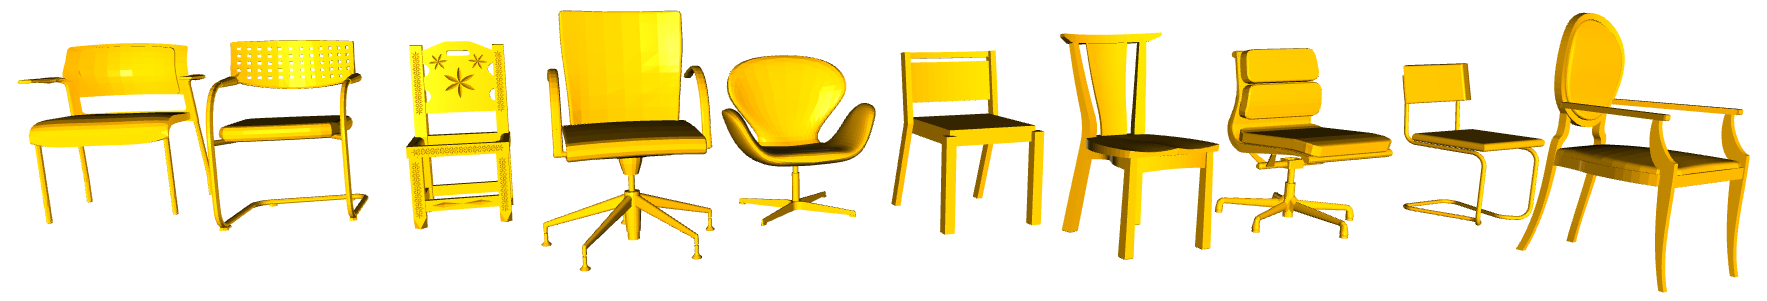
\includegraphics[width=\textwidth]{resources/chairs.png}
                 \caption{Chairs}
                 \label{fig:chairs}
             \end{subfigure}
             \begin{subfigure}[b]{\textwidth}
                \addtocounter{subfigure}{-1}
                \renewcommand\thesubfigure{\alph{subfigure}.II}
                 \centering
                 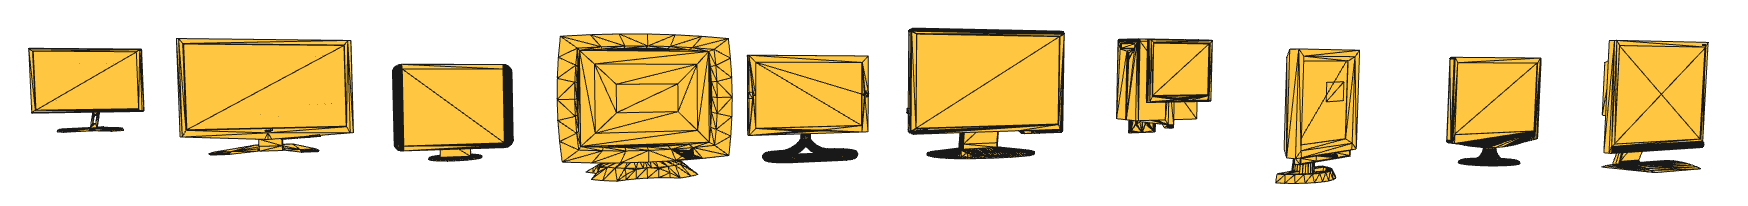
\includegraphics[width=\textwidth]{resources/monitor.png}
                 \caption{Monitors}
                 \label{fig:monitors}
             \end{subfigure}
            \addtocounter{subfigure}{-1}
            \caption{Example of (\ref{fig:chairs}) Chairs and (\ref{fig:monitors}) Monitors samples from \mbox{ModelNet10} dataset.}
            \label{fig:CADModels}
            \addtocounter{subfigure}{+1}
        \end{subfigure}
        \begin{subfigure}{0.10\textwidth}
        \end{subfigure}
        \begin{subfigure}{0.45\textwidth}
            %\renewcommand\thesubfigure{\alph{subfigure}.}
            \centering
             \begin{subfigure}[b]{\textwidth}
                \addtocounter{subfigure}{-1}
                \renewcommand\thesubfigure{\alph{subfigure}.I}
                 \centering
                 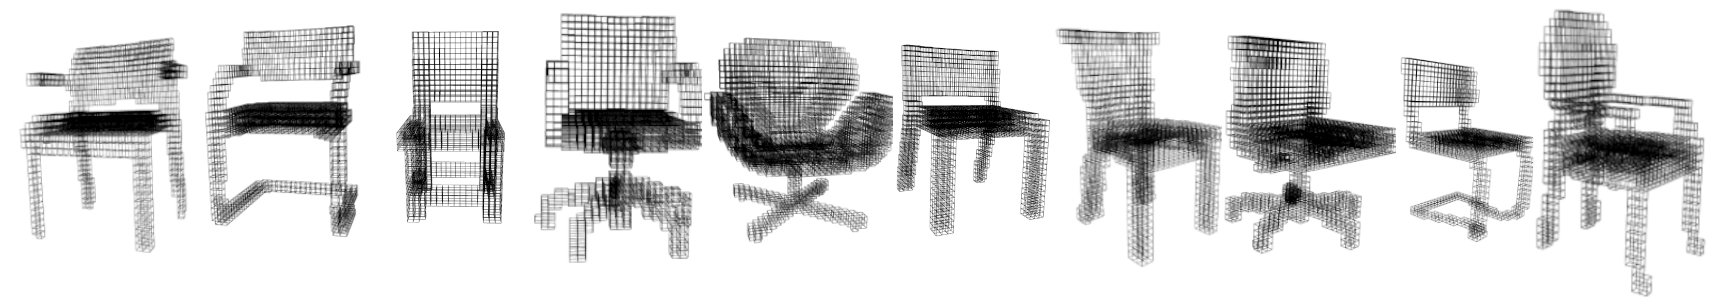
\includegraphics[width=\textwidth]{resources/chairs_voxels.png}
                 \caption{Chairs}
                 \label{fig:chairsVoxels}
             \end{subfigure}
             \begin{subfigure}[b]{\textwidth}
                \addtocounter{subfigure}{-1}
                \renewcommand\thesubfigure{\alph{subfigure}.II}
                 \centering
                 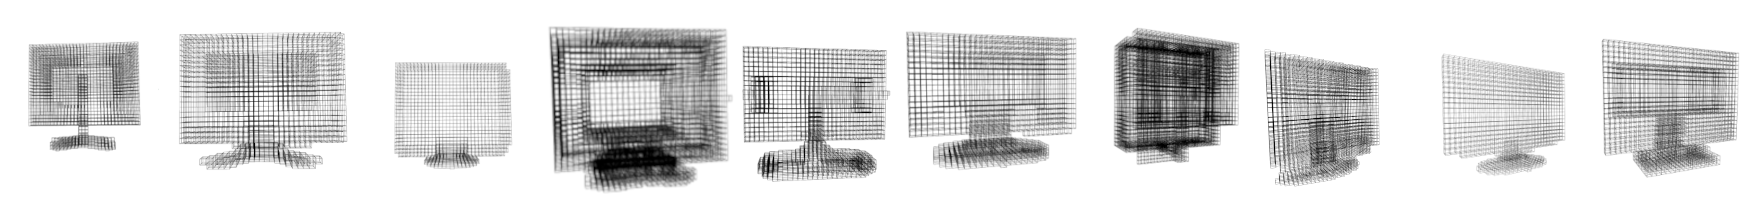
\includegraphics[width=\textwidth]{resources/monitors_voxels.png}
                 \caption{Monitors}
                 \label{fig:monitorsVoxels}
             \end{subfigure}
            \addtocounter{subfigure}{-1}
             
            \caption{Example of voxelized (\ref{fig:chairsVoxels}) Chairs and (\ref{fig:monitorsVoxels}) Monitors samples of Figure \ref{fig:CADModels}}
            \label{fig:VoxelizedModels}
        \end{subfigure}
        \caption{Examples of Chairs and Monitors samples. Fig.~\ref{fig:CADModels} shows the original CAD models, and Fig.~\ref{fig:VoxelizedModels} the voxelized versions of them.} 
        \label{fig:samples}
    \end{center}
\end{figure*}
\section{Processing Pipeline}
\label{sec:pipeline}

In this part, we explain our methodology, starting with the dataset preparation and giving some insights on our classifiers.\\

\textbf{Dataset preparation}
In the field of machine learning, the availability and quality of training data play a crucial role in determining the performance and generalizability of models. The original dataset we used as starting point, ModelNet10, comes as a clean collection of 3D CAD models for 10 classes of objects.
The owner has cleaned and manually aligned the orientations of the models, but they are not scaled nor \ac{IID}.

As the initial entries were CAD models, we had to translate them into voxel grids in order to use with 3D Neural Networks. 
%We used Open3d, a Python library, for the conversion, and then we normalized the grids.

To solve the unbalanced problem in the distribution of the samples, we choose to augment our data with Rotations. \\
%Fig.~\ref{fig:rotatedChair} shows an example of different rotations of the first chair in Fig.~\ref{fig:chairs}.
Rotations in our task has several advantages, e.g.: 
\begin{itemize}
    \item rotations helps our model to learn a stronger model that can recognize an object from different positions;
    \item data augmentation helps us to have more data to train our models;
    \item picking different number of rotations per category, depending on its initial distribution, we are able to balance the samples among the classes. More details in Sec. \ref{sec:dataset}.
\end{itemize}

%From Fig.~\ref{fig:finalTrainSetDistribution} we can see that the dataset becomes well-balanced with rotations.

%OLD: So we augmented the data with rotations, the methodology is explained in Sec. \ref{sec:dataset}, and using this approach we managed to arrive at a dataset with identically distributed classes.

We decided to store the rotated dataset efficiently as voxel grids, and start from this for the training. This allowed us to save a considerable amount of computation time, thus leaving only the transformation of those stored voxel grids into Binary Voxels (BV), required by the model.\\

Inspired by RandomErasing \cite{zhong2017random} and \cite{devries2017improved} , the cutout, 3d version of it, is applied to the sample during training. Cutout is a Data Augmentation technique which randomly masking out regions of the input data.
In our process, with a probability of 20\%, cutout removes a randomly selected 8x8x8 cube from the sample, by putting the voxel contained in this region to 0. This kind of technique encourage the network to learn more robust and general features and reduce overfitting. 
\\

\textbf{Models, Training and Evaluation}
As our baseline model for the classification, we started with a simple 3D CNN backbone followed by a fully connected layer. 
Initially, we choose to train the model on a smaller dataset to check if it was powerful enough to overfit, or we needed to increase the depth. Very soon the model overfitted it, thus we stick with the model for further improvements.\\
In order to make the model learn more general features, we used 3D Cut-Out technique, which improved the results of the baseline model.
The best result we get is with our bagging classifier, an ensemble of 5 baseline models trained on different partitions of the dataset. More details on partitioning in Sec.~\ref{sec:dataset} and on the classifier in Sec.~\ref{sec:learning_framework}.\\

Fig.~\ref{fig:pipeline} shows the training pipeline. We can see that for each weak model, we have a different partition, whereas during the evaluation phase, we used the test partition of the entire dataset.

%Then, we trained the 5 models that compose the bagging system on the entire dataset.
%We obtained 5 models, trained in different dataset, and at the end, we created a function which composes the predicted guess of all the 5 models to give as output the final prediction.

% TODO move to LF
%Each of the five weak classifier consists of two parts, 3D CNN backbone followed by a fully connected multi-layer neural network.

% Once we have obtained a Dataset of voxel grids we start the analysis and the creation of our models. The first thing we have to do is to read in memory the voxel from the dataset, each sample is represented as a list of coordinates of each non-empty voxel. We transform them into 3D boolean arrays of size 32x32x32 where each cell is true if and only if in such a position the associated voxel has a block on that grid. The spatial relationship is represented correctly with this data structure, but it increases the amount of memory required.


% Once the data are ready and in the correct shape what we need to do is to train our model. 
%We first tried to train our model with a smaller dataset to check if our network was powerful enough to overfit, or if we needed to increase the depth.
%Then, we trained the 5 models that compose the bagging system on the entire dataset.
%We obtained 5 models, trained in different dataset, and at the end, we created a function which composes the predicted guess of all the 5 models to give as output the final prediction.

  

% [TODO:https://arxiv.org/pdf/1901.08373.pdf:
% For the feature of every voxel, the simple
% Binary Voxel (BV) method is used to treat it as a binary value.
% The value 1 is assigned to the feature if there exists a point
% in corresponding voxel, otherwise, the voxel is empty and the
% feature value is 0. The drawback of this method is that the
% local shape information of points within a voxel is lost. To
% avoid the loss of local information, the voxel size in the BV
% is usually set very small to generate high-resolution 3D grids;

% An alternative method is to use PointNet [24] to extract the
% pointwise features, which is called Voxel Feature Encoding
% (VFE) [30]. It enables inter-point interaction within a voxel
% by combining pointwise features with a locally aggregated
% feature, which can help to learn the local 3D shape information, and hence, can alleviate information loss due to data
% quantization. Since VFE requires a number of points per valid
% voxel, the voxel size in VFE should be large. 
% ]

%Then we used a cutout technique to set a portion of size 8x8x8 to a determined number (20\%) of samples: Cutout is a Data Augmentation technique, one of the main benefits of Cutout is that it forces the model to learn to ignore irrelevant features in the input data, which can make the model more robust to unseen variations in the test data, but it can be a double-edged sword, so it must be used correctly otherwise it may reduce the performance of the model. Last we create and train our Convolutional neural network, it is composed by two Convolutional 3D layers, each of them followed by a Map Pooling, and the last two layers are dense, the output is an array of length 10, equal to the number of class in the dataset. 
%
